% ============================================================================
%  硕士学位论文开题报告及论文工作计划 —— 张家艺（219 1.5 μm 单端 TDLAS）
%  编译：xelatex（UTF-8）；字体：Fandol（宋体/黑体/楷体/仿宋）
%  正文节次按学校《硕士学位论文开题报告及论文工作计划》模板组织
%  2026-10-30 定稿（草稿 v2 确认版）
% ============================================================================
\documentclass[12pt,a4paper]{article}
\usepackage{fontspec}
\usepackage{geometry}
\usepackage{tikz}
\usepackage{multirow}
\usepackage{booktabs}
\usepackage{longtable}
\usepackage{array}
\usepackage{graphicx}
\usepackage{caption}
\usepackage{amsmath}
\usetikzlibrary{arrows.meta,positioning}

% ---------------- 中文字体（Fandol，自 texmf-local 加载） ----------------
\newcommand{\zhfontdir}{/home/xliu/data/219-1.5um-TDLAS/1-publication/开题报告-2026/texmf-local/fonts/opentype/public/fandol/}
\setmainfont{FandolSong-Regular.otf}[Path=\zhfontdir, BoldFont=FandolSong-Bold.otf]
\newfontfamily{\heiti}{FandolHei-Regular.otf}[Path=\zhfontdir]
\newfontfamily{\kaiti}{FandolKai-Regular.otf}[Path=\zhfontdir]
\newfontfamily{\fangsong}{FandolFang-Regular.otf}[Path=\zhfontdir]

% ---------------- 页面与段落设置 ----------------
\geometry{a4paper, top=2.5cm, bottom=2.5cm, left=3.0cm, right=2.5cm}
\setlength{\parindent}{2em}
\setlength{\parskip}{0.4em}
\linespread{1.35}

% 章节标题：黑体，居中或左对齐
\usepackage{titlesec}
\titleformat{\section}{\heiti\large}{\thesection}{1em}{}
\titleformat{\subsection}{\heiti\normalsize}{\thesubsection}{1em}{}
\titleformat{\subsubsection}{\heiti\normalsize}{\thesubsubsection}{1em}{}

% 表格标题样式
\captionsetup{font=small,labelfont=bf}

\newcommand{\ch}{\textsuperscript{注：}}

\begin{document}

% ============================================================================
%  封面
% ============================================================================
\thispagestyle{empty}
\begin{center}
  \vspace*{1.2cm}
  {\heiti\LARGE 山东科技大学}\\[0.8em]
  {\heiti\LARGE 硕士研究生学位论文开题报告}\\[0.4em]
  {\heiti\LARGE 及论文工作计划}\\[2.0em]

  \renewcommand{\arraystretch}{1.9}
  \begin{tabular}{|>{\heiti}p{4.2cm}|p{10.5cm}|}
    \hline
    论文题目 & {\kaiti 面向燃煤锅炉与煤炭原位开采的 1.5\,$\mu$m}\\
             & {\kaiti 单端 TDLAS 测温方法研究}\\
    \hline
    研究生姓名 & 张家艺\\
    \hline
    导师姓名、职称 & 刘训臣 \ 教授\\
    \hline
    学科、专业 & 机械\\
    \hline
    研究方向 & 热流体激光诊断与测量\\
    \hline
    入学年月 & 2025 年 9 月\\
    \hline
    所属学院 & 机械电子工程学院\\
    \hline
    开题时间 & 2026 年 \ \ \ \ 月 \ \ \ \ 日\\
    \hline
  \end{tabular}\\[2.2em]

  {\fangsong\large 山东科技大学学位评定委员会办公室制表}
\end{center}
\clearpage

% ============================================================================
%  一、立论依据
% ============================================================================
\section{立论依据}

\subsection{课题来源、选题依据和立论背景}

\textbf{课题来源。}本课题依托课题组深部煤炭原位流态化开采（711）项目与燃煤锅炉（343）应用方向，面向两者共同的在线测温需求，开展 1.5\,$\mu$m 单端 TDLAS（可调谐半导体激光吸收光谱）测温方法研究。

\textbf{温度是燃烧过程最核心的状态参数。}燃煤锅炉的燃烧效率、污染物生成与运行安全，煤炭地下气化的反应路径与转化率，都由温度场直接决定——在线、准确、非接触的温度测量是这两类重大需求的共性瓶颈。

\textbf{两大应用场景提出同一类测量难题。}一是煤粉锅炉：炉膛高温（1500--1750\,K）、高粉尘、强振动，传统测点难以长期服役；二是深部煤炭原位流态化开采（谢和平院士提出的"11+X"技术体系）：地下 10--25\,MPa 高温高压、高水蒸气/CO$_2$ 活性气氛中，煤热解气化的动力学研究急需原位激光诊断手段。

\textbf{传统测温手段在两类场景下均受限。}热电偶属接触式测量：热惯性大、易烧蚀、需逐点安装，且在高粉尘气流中寿命短；辐射测温与火焰成像依赖发射率假设，反演不确定度大；透射式 TDLAS 虽成熟，但需要在被测对象两侧各开一个光学窗口——锅炉炉墙与井下高压反应器往往只允许单侧开孔安装，双侧透射方案在现场难以落地。

\textbf{单端（single-ended）TDLAS 是解决"只能装一侧"问题的直接途径。}发射与接收共用同一侧光路，光束打到测量区尾端的反射面后折回接收，只需单侧窗口。其代价是回波信号弱、发射光背景强，对光路设计与接收链路提出更高要求——这正是本课题的方法学出发点。

\textbf{1.5\,$\mu$m 通信波段为单端 TDLAS 的工程化提供了器件红利。}H$_2$O 在 1.4--1.5\,$\mu$m 有可用的吸收带；该波段处于光纤通信窗口，MEMS 可调谐 VCSEL、EDFA 光纤放大器、InGaAs APD 等器件成熟且成本低、全光纤化鲁棒性好——相比中红外（QCL/带间级联）方案，具备显著的工程化与现场部署优势。

\subsection{课题研究目的、理论意义和实际应用价值}

\textbf{研究目的。}研制一套 1.5\,$\mu$m 单端 TDLAS 测温系统并完成三级应用验证：系统实现 100\,kHz 波长扫描、亚毫秒级温度反演；在 crossflow 燃烧平台完成尾端反射与横向火焰双模式实验室验证；在燃煤锅炉现场完成工程化测量；探索与煤炭原位流态化开采高温高压反应器的耦合应用。

\textbf{理论意义。}发展一套基于电信级器件的 1.5\,$\mu$m 单端 TDLAS 测温方法，实现高频扫描（100\,kHz）与亚毫秒级温度反演，形成"单侧安装、全光纤、低成本、高鲁棒"的高温气体测温新手段，并研究高温高压展宽条件下的双线选择与反演精度问题，为单端架构在工程现场的定量测温提供方法学依据。

\textbf{实际应用价值。}打通"实验室缩比验证 $\rightarrow$ 燃煤锅炉现场测量 $\rightarrow$ 煤炭原位开采高温高压应用"三级应用场景，为锅炉燃烧优化与深部煤炭原位气化的动力学研究提供在线温度数据。本课题属课题组"2xx 诊断技术 $\rightarrow$ 3xx 平台应用"研究体系中的方法线（219 单端 TDLAS），成果直接支撑锅炉（343）与原位开采（711）两条应用线，并可移植至多路层析（215）等相关系统。

% ============================================================================
%  二、文献综述
% ============================================================================
\section{文献综述}

\subsection{国内外研究现状、发展动态}

\textbf{TDLAS 气体测温技术概述。}TDLAS 以 Beer--Lambert 定律为基础，是非接触、物种选择、快响应的燃烧诊断主流手段。双线比值法选取两条低态能量差较大的吸收线，由吸收比值直接反演温度，无需标定组分浓度（Goldenstein 等 2017 年综述\cite{goldenstein2017}）。经过数十年发展，TDLAS 已从实验室走向工业现场，但在煤粉锅炉等大型设备上仍以透射式布置为主。

\textbf{单端 TDLAS 研究进展。}单端架构的核心思想是"发射--接收同侧、反射面折返"，近十年在国际上快速发展：
\begin{itemize}
  \item Melin 等（2017）系统研究了单端回射（retroreflection）传感器的反射面选择与高温环境适应性，为反射面材质与结构提供了设计依据\cite{melin2017}；
  \item Zhou、Mathews、Goldenstein（2018）提出紧凑型光纤耦合单端传感器，将单端光路全光纤化，显著提升了工程鲁棒性\cite{zhou2018}；
  \item Peng 等（2016）研制中红外单端传感器，实现 H$_2$O/CO$_2$/CO 与温度的同时测量\cite{peng2016}；（2019a）将单端传感器用于激波管，实现测温与组分测量的单次通过\cite{peng2019a}；（2019b）面向旋转爆震发动机环腔，实现了高温高压下 H$_2$O 浓度与温度的时间分辨测量\cite{peng2019b}——表明单端方案已通过极端环境考核；
  \item Hansemann 等（2024）发展了空间分辨的单端 TDLAS 系统，把单点测量推进到沿程分布测量\cite{hansemann2024}；
  \item Luo 等（2024）在分层旋流燃烧器下游完成单端 TDLAS 温度测量，展示了真实燃烧装置上的应用能力\cite{luo2024}。
\end{itemize}

\begin{table}[htbp]
  \centering
  \caption{单端 TDLAS 代表性文献对比}
  \begin{tabular}{lllll}
    \toprule
    文献 & 波段 & 应用场景 & 反射/回波方案 & 主要指标 \\
    \midrule
    Melin 2017\cite{melin2017} & 近红外 & 高温环境原理验证 & 回射面 & 反射面选型依据 \\
    Zhou 2018\cite{zhou2018} & 1.4/1.5\,$\mu$m & 紧凑型传感器 & 光纤耦合单端 & 小型化、全光纤 \\
    Peng 2016/2019\cite{peng2016,peng2019a,peng2019b} & 中红外 & 多组分/激波管/RDE & 单端回波 & H$_2$O/CO$_2$/CO/T 同测 \\
    Hansemann 2024\cite{hansemann2024} & 近红外 & 空间分辨测量 & 单端多角度 & 沿程分布 \\
    Luo 2024\cite{luo2024} & 近红外 & 旋流燃烧器 & 单端 & 真实火焰测温 \\
    本文 & 1.5\,$\mu$m & 锅炉现场 + 原位开采高压 & 裸光纤端面/环形器替代 & 100\,kHz 扫描、亚毫秒反演 \\
    \bottomrule
  \end{tabular}
\end{table}

\textbf{小结：}现有单端工作集中在中红外波段或实验室原理验证，面向燃煤锅炉现场与煤炭原位开采高压环境的 1.5\,$\mu$m 电信级单端系统尚属空白——这是本课题的切入点之一。

\textbf{1.5\,$\mu$m 波段与 VCSEL 光源进展。}MEMS 可调谐 VCSEL 兼具宽调谐与高扫描频率。商用 1550\,nm MEMS-VCSEL 驱动调制带宽达 200\,kHz、单次完整波长扫描约 10\,$\mu$s（100\,kHz），远快于传统 DFB 波长扫描；配合 EDFA 可补偿链路损耗，配合通信级 InGaAs APD 可实现高灵敏度接收。电信产业链使 1.5\,$\mu$m 系统成本与可靠性显著优于中红外方案，但其在高温燃烧测温中的系统级应用研究仍较少。

\textbf{燃煤锅炉与煤气化场景的激光诊断应用现状。}燃煤电厂侧已有透射式 TDLAS 的成功先例：Chao、Jeffries、Hanson（2013）用 2.3\,$\mu$m 传感器实现燃煤电厂 CO 的实时在线监测\cite{chao2013}；Li 等（2020）开发了脱硝过程 NH$_3$/H$_2$O/温度同时测量的便携 robust 传感器\cite{li2020}；大型煤粉炉温度场方面，Zhou 等（2005）实现炉膛三维温度场可视化\cite{zhou2005}，Wang 等（2020）将 CT-TDLAS 用于燃煤炉二维测温\cite{wang2020}，Li 等（2024）用火焰图像处理获得大型煤粉炉温度与吸收系数二维分布\cite{li2024}。

煤气化侧：Ouyang 等（1998）研制了加压下落管炉用于煤反应性研究\cite{ouyang1998}；Sun 等（2013）在犹他大学高压携带流气化炉上发展 TDLAS 传感器，实现高温高压含尘气流中气体温度与浓度的测量\cite{sun2013}；Sun 等（2014）进一步将波长扫描 WMS 应用于工程级高压煤气化炉的 H$_2$O 在线测量\cite{sun2014}。

\textbf{小结：}现场应用以透射式/层析式/成像式为主，均需双侧窗口或大型系统；单端方案在锅炉与煤气化现场的应用报道极少——本课题的应用创新空间所在。

\textbf{现状总结。}综合以上进展，存在三个明确缺口：其一，1.5\,$\mu$m 电信级器件单端 TDLAS 的系统级工程化；其二，真实火焰、高粉尘现场环境下的单端回波验证；其三，单端测温与煤炭原位开采高温高压反应器（蓝宝石棒状窗口）的耦合应用。本课题针对这三个缺口展开。

\subsection{所阅文献的查阅范围及手段}

通过 Web of Science / Scopus / 课题组 Zotero 文献库（编号 tag 21x/34x/71x 段位）检索 TDLAS 测温、单端/反射式激光吸收、MEMS-VCSEL 与 1.5\,$\mu$m 波段诊断、燃煤锅炉与煤气化激光在线监测等主题文献，重点精读单端架构原理、反射面与光路设计、高温高压展宽处理三类文献，形成以上综述。主要参考文献列于文末。

% ============================================================================
%  三、研究内容、技术路线、创新点
% ============================================================================
\section{研究内容、技术路线、创新点}

\subsection{主要研究内容及拟解决的关键技术}

\textbf{研究内容一：1.5\,$\mu$m 波段光谱仿真与吸收线优选。}基于 HITRAN/HAPI 数据库，对 6410--6493\,cm$^{-1}$（1.540--1.560\,$\mu$m）波段在锅炉主燃区工况（1500\,$^\circ$C、常压微负压、16\,m 光程）下的 H$_2$O 多线吸收光谱进行 Voigt 线型仿真与仪器展宽处理；面向 1550--1750\,K 温区开展双线组合优化（低态能量差、吸收强度、邻峰干扰三准则），完成信噪比与温度灵敏度预估，输出选线数据库。

\textbf{研究内容二：单端 TDLAS 硬件系统研制。}包括：VCSEL+EDFA 光源链路（100\,kHz 扫描、调谐线性化）；单端收发光路——环形器方案与"裸光纤端面反射替代"方案的对比实施，收发隔离与背景抑制；接收链路——InGaAs APD（25--175\,V 偏置）+ 高带宽 TIA（OPA855，闭环带宽约 500\,MHz）+ 1500/1600\,nm 带通滤波（抑制 980\,nm 泵浦光与炉膛背景辐射）；数据采集与波长标定。

\textbf{研究内容三：crossflow 平台实验室验证。}在横向射流燃烧平台开展双模式验证：尾端反射模式（燃烧器尾端/侧壁安装反射镜或漫反射板，收集沿烟气路径回波，验证长光程烟气测温）与横向火焰模式（光束穿越第一级火焰反应区，采集高温 H$_2$O 吸收）；完成温度反演与热电偶对比、信噪比与不确定度分析。

\textbf{研究内容四：燃煤锅炉现场应用研究。}依托校外集装箱试验场地与电站合作（343 线）：探头吹扫防污与防尘设计、减振安装、工控机一体化集成与现场数据采集流程，开展炉膛/烟道实测温，评估现场工况下系统长期稳定性。

\textbf{研究内容五：煤炭原位开采高温高压应用探索。}依托 711 高压固定床/流动管反应器（内筒 $\phi$220$\times$15、允许工作压力 17.3\,MPa、10 段独立控温至 1000\,$^\circ$C）：设计蓝宝石棒状光学窗口（$\phi$8$\times$50\,mm、锥面密封+主动水冷法兰）与单端探头接口，研究高水蒸气/CO$_2$ 气氛、10--25\,MPa 压力展宽条件下的谱线模型修正与温度反演方法。

\textbf{拟解决的关键科学与技术问题：}
\begin{enumerate}
  \item \textbf{单端构型下的收发隔离与弱回波提取：}发射端强背景与光纤端面杂散反射比有效回波高若干量级，需通过光路设计（环形器/收发分离/分束方案比选）、滤波与调制解调手段提取微弱回波。
  \item \textbf{高温高压展宽下的双线选择与反演精度：}锅炉高温与原位开采高压（谱线压力展宽显著）工况下，双线组合与谱线参数（碰撞展宽系数及其温度依赖）直接决定反演不确定度，需仿真--实验联合修正。
  \item \textbf{现场工况的工程适应性：}粉尘沉积与窗口污染、机械振动、安装空间受限、电磁干扰等现场因素下的长期稳定测量方案（吹扫、减振、屏蔽、标定流程）。
\end{enumerate}

\subsection{拟采取的研究方法、技术路线、实施方案及可行性分析}

\textbf{研究方法——双线比值法测温。}选取 H$_2$O 两条吸收线，由 Beer--Lambert 定律测得积分吸收 $A_1$、$A_2$，其比值 $R$ 仅依赖温度：
\begin{equation}
  T = \frac{\Delta E}{k\left[\ln R + \ln\frac{S_1(T_0)}{S_2(T_0)}\right]}
\end{equation}
其中 $\Delta E$ 为两条吸收线低态能量差，$S_i(T_0)$ 为参考温度 $T_0$ 下的线强，$k$ 为玻尔兹曼常数。

\textbf{光谱仿真方法：}Python + HAPI（HITRAN API），Voigt 线型吸收系数计算 $\rightarrow$ 透射/吸收/辐射光谱 $\rightarrow$ 高斯卷积模拟仪器展宽（FWHM 0.5\,cm$^{-1}$），波数步长 0.005\,cm$^{-1}$；工况按应用对象设置（锅炉：1773\,K、0.999\,atm、16\,m 光程；原位开采：变压力 1--25\,MPa 参数化扫描）。

\textbf{实验方法：}直接吸收为主、预留波长调制（WMS）升级；100\,kHz 扫描时序由函数发生器统一触发采集；标定采用热电偶对比与标准火焰/黑体源。

\textbf{技术路线：}

\begin{center}
\begin{tikzpicture}[
  node distance=4mm and 6mm,
  box/.style={draw, rounded corners=1.5mm, align=center, inner sep=2.2mm, font=\small},
  arrow/.style={-{Stealth[length=2.6mm]}, thick}
]
  \node[box] (s1) {光谱仿真与选线\\（HAPI，锅炉/高压双工况）};
  \node[box, below=6mm of s1] (s2) {单端 TDLAS 系统研制\\光源链路（VCSEL+EDFA）$\rightarrow$ 单端光路（环形器/端面反射）\\$\rightarrow$ 接收链路（APD+OPA855+带通滤波）$\rightarrow$ 采集与波长标定};
  \node[box, below=6mm of s2] (s3) {crossflow 平台实验室验证\\（尾端反射 + 横向火焰双模式）};
  \node[box, below=6mm of s3] (s4) {燃煤锅炉现场应用\\（集装箱场地 $\rightarrow$ 电站实测）};
  \node[box, right=6mm of s4] (s5) {原位开采高压应用\\（蓝宝石窗口 + 高压反应器耦合实验）};
  \node[box, below=6mm of s4] (s6) {数据库、论文、专利产出};
  \draw[arrow] (s1) -- (s2);
  \draw[arrow] (s2) -- (s3);
  \draw[arrow] (s3) -- (s4);
  \draw[arrow] (s4) -- (s6);
  \draw[arrow] (s4.east) -- (s5.west);
  \draw[arrow] (s5.south) |- (s6.east);
\end{tikzpicture}
\end{center}

\textbf{可行性分析：}
\begin{itemize}
  \item \textbf{器件可行——核心器件全部到位并完成出光验证：}MEMS-VCSEL（$>$1\,mW、100\,kHz 扫描已验证）、EDFA（操作流程已标准化）、1500/1600\,nm 滤波片（到货验收合格）、APD 与光接收模块（已到货）、OPA855 高带宽 TIA 模块（已下单）；带宽需求已完成定量论证（100\,kHz 扫描需约 440\,MHz $\rightarrow$ OPA855 闭环约 500\,MHz 覆盖，低速模式 150\,MHz 模块亦有 3 倍余量），带宽瓶颈已正式关闭。
  \item \textbf{仿真可行——选线依据已具备：}1.5\,$\mu$m 波段锅炉工况仿真（1773\,K、0.999\,atm、16\,m 光程）已完成并归档，吸收峰识别与邻峰间距统计已开展。
  \item \textbf{平台可行：}实验室 crossflow 燃烧平台可用；校外集装箱试验场地已建立（激光系统已进场）；711 反应器加热段设计已按 GB/T 20801 GC1 级定稿（水压试验 22.5\,MPa），蓝宝石棒状窗口方案已定，法兰已加工到货，10 段独立温控方案落地中。
  \item \textbf{团队可行：}课题组在 TDLAS 方向有系统积累（215 多路层析成像、216 反射式 TDLAS、217 中红外痕量组分、212 双线测温），可为本课题提供光路设计、光谱反演与硬件调试支撑；711 项目与中煤集团合作（校外导师刘舆帅教授），应用场景有保障。
  \item \textbf{个人基础可行：}本人承担 215 项目第二负责人（多路 TDLAS 层析，负责窗口框架统筹出图）、711 项目负责人（反应器装置设计定稿）、704 煤粉红外遥测负责人，已完成本课题全部前期硬件与仿真工作（见第四节）。
  \item \textbf{风险与对策：}APD 首次调试疑似偏压不当损坏 $\rightarrow$ OPA855 模块到货后按"暗电流先行"流程复测，必要时补购；现场上位机连接问题 $\rightarrow$ 按导师既定路径以"已验证整机"替换排查；高压窗口密封风险 $\rightarrow$ 沿用 711 已定稿的锥面密封+紫铜垫圈+主动水冷方案并预留盲板。
\end{itemize}

\subsection{论文的创新点}

\textbf{创新点一（系统层面）：}提出基于电信级器件的 1.5\,$\mu$m 全光纤单端 TDLAS 测温系统——VCSEL+EDFA+APD 通信波段器件链 + 单端回波光路，实现"单侧安装、低成本、高鲁棒"，区别于现有中红外单端方案，面向锅炉炉墙与井下受限空间的工程部署。

\textbf{创新点二（测量性能层面）：}MEMS-VCSEL 100\,kHz 快速扫描与约 500\,MHz 高带宽接收链路结合，实现亚毫秒级温度反演，具备分辨燃烧不稳定特征的时间分辨率；完成从经验估算到仿真精算的接收带宽定量设计方法。

\textbf{创新点三（应用场景层面）：}首次将单端 TDLAS 与深部煤炭原位流态化开采高温高压反应器耦合——蓝宝石棒状窗口（锥面密封+主动水冷）单侧接口设计，支撑 10--25\,MPa 活性气氛下煤热解气化的原位温度诊断；同步打通燃煤锅炉现场应用链路。

% ============================================================================
%  四、研究基础
% ============================================================================
\section{研究基础}

\subsection{所需实验手段、研究条件和实验条件}

\textbf{所需实验手段：}1.5\,$\mu$m 单端 TDLAS 测温系统（VCSEL+EDFA+环形器/端面反射+APD 接收链路）、HITRAN/HAPI 光谱仿真、crossflow 燃烧平台、热电偶标定、红外相机辅助对准。

\textbf{研究条件：}课题组 223 实验室（光学平台、燃烧平台、函数发生器与示波器等测量仪器）、校外集装箱试验场地（343 线）、711 高压反应器（内筒 $\phi$220$\times$15、允许工作压力 17.3\,MPa、10 段独立控温）。

\textbf{所需经费（含经费来源、开支预算）：}经费来源为课题组项目经费（711/343）。主要开支预算如下（单位为元，价格为采购/询价参考值，以实际采购为准）：

\begin{table}[htbp]
  \centering
  \caption{主要设备与经费预算（估算）}
  \begin{tabular}{lll}
    \toprule
    设备/项目 & 数量 & 预算（元） \\
    \midrule
    1550\,nm MEMS-VCSEL 激光器 & 1 & 已采购 \\
    EDFA 光纤放大器 & 1 & 已采购 \\
    InGaAs APD 与光电接收模块 & 1 套 & 已采购 \\
    1500/1600\,nm 带通滤波片 & 各 1 & 已采购 \\
    OPA855 高带宽 TIA 模块 & 1 & 已下单 \\
    环形器与光纤跳线等光路件 & 若干 & 待采购 \\
    工控机与数据采集 & 1 & 已有 \\
    加工与安装件 & 若干 & 约 5000 \\
    实验耗材（气瓶等） & 若干 & 约 10000 \\
    \bottomrule
  \end{tabular}
\end{table}

\subsection{前期工作基础}

\textbf{系统硬件已基本齐备（对应研究内容二）：}完成 VCSEL 激光器上架、首次上电调试与出光验证（$>$1\,mW，扫描特性经供应商确认）；EDFA 安装与标准操作流程（SOP）固化；滤波片选型采购验收（1500\,nm HP + 1600\,nm LP 组合，可阻挡 980\,nm 泵浦光与 $>$1600\,nm 背景辐射）；APD 探测系统选型（带宽需求经三步定量估算）；2026-09 完成机柜整合与激光器金属盒静电屏蔽封装（图~\ref{fig:cabinet}）。

\begin{figure}[htbp]
  \centering
  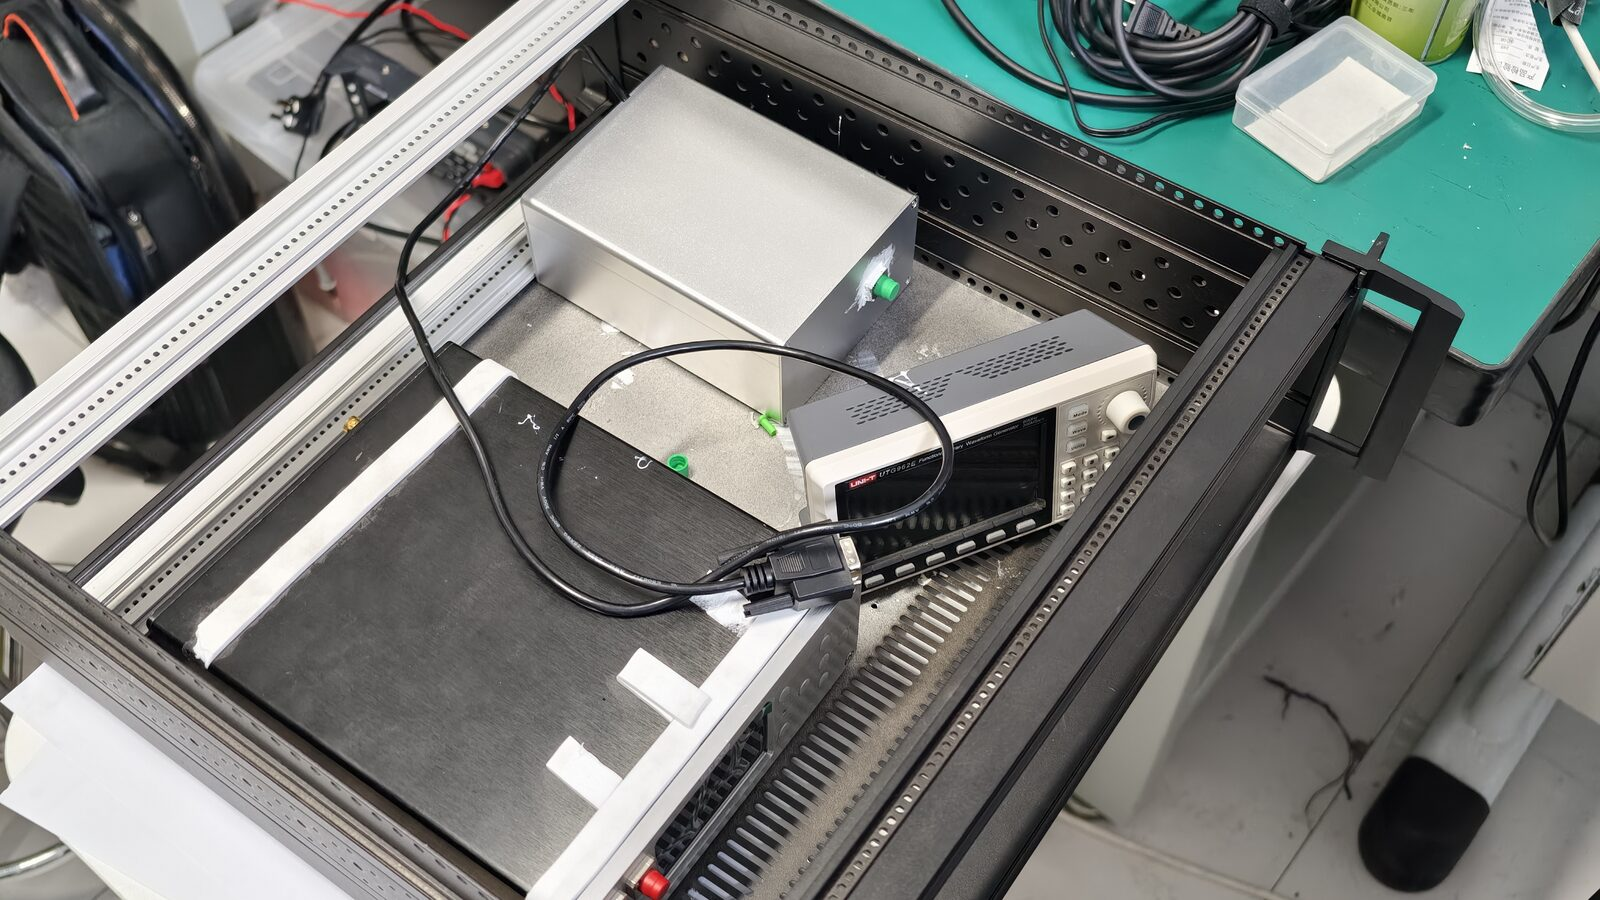
\includegraphics[width=0.62\textwidth]{figures/20260918-机柜固定与激光器金属盒封装.jpg}
  \caption{机柜固定与激光器金属盒封装（2026-09-18）}
  \label{fig:cabinet}
\end{figure}

\textbf{光谱仿真已完成首轮（对应研究内容一）：}HAPI 仿真输出吸收系数、透射、吸收、辐射四合一光谱数据（6 个数据文件+图，图~\ref{fig:spectra}），仿真参数与锅炉主燃区工况匹配；吸收峰识别与邻峰间距统计支撑了接收带宽精算。

\begin{figure}[htbp]
  \centering
  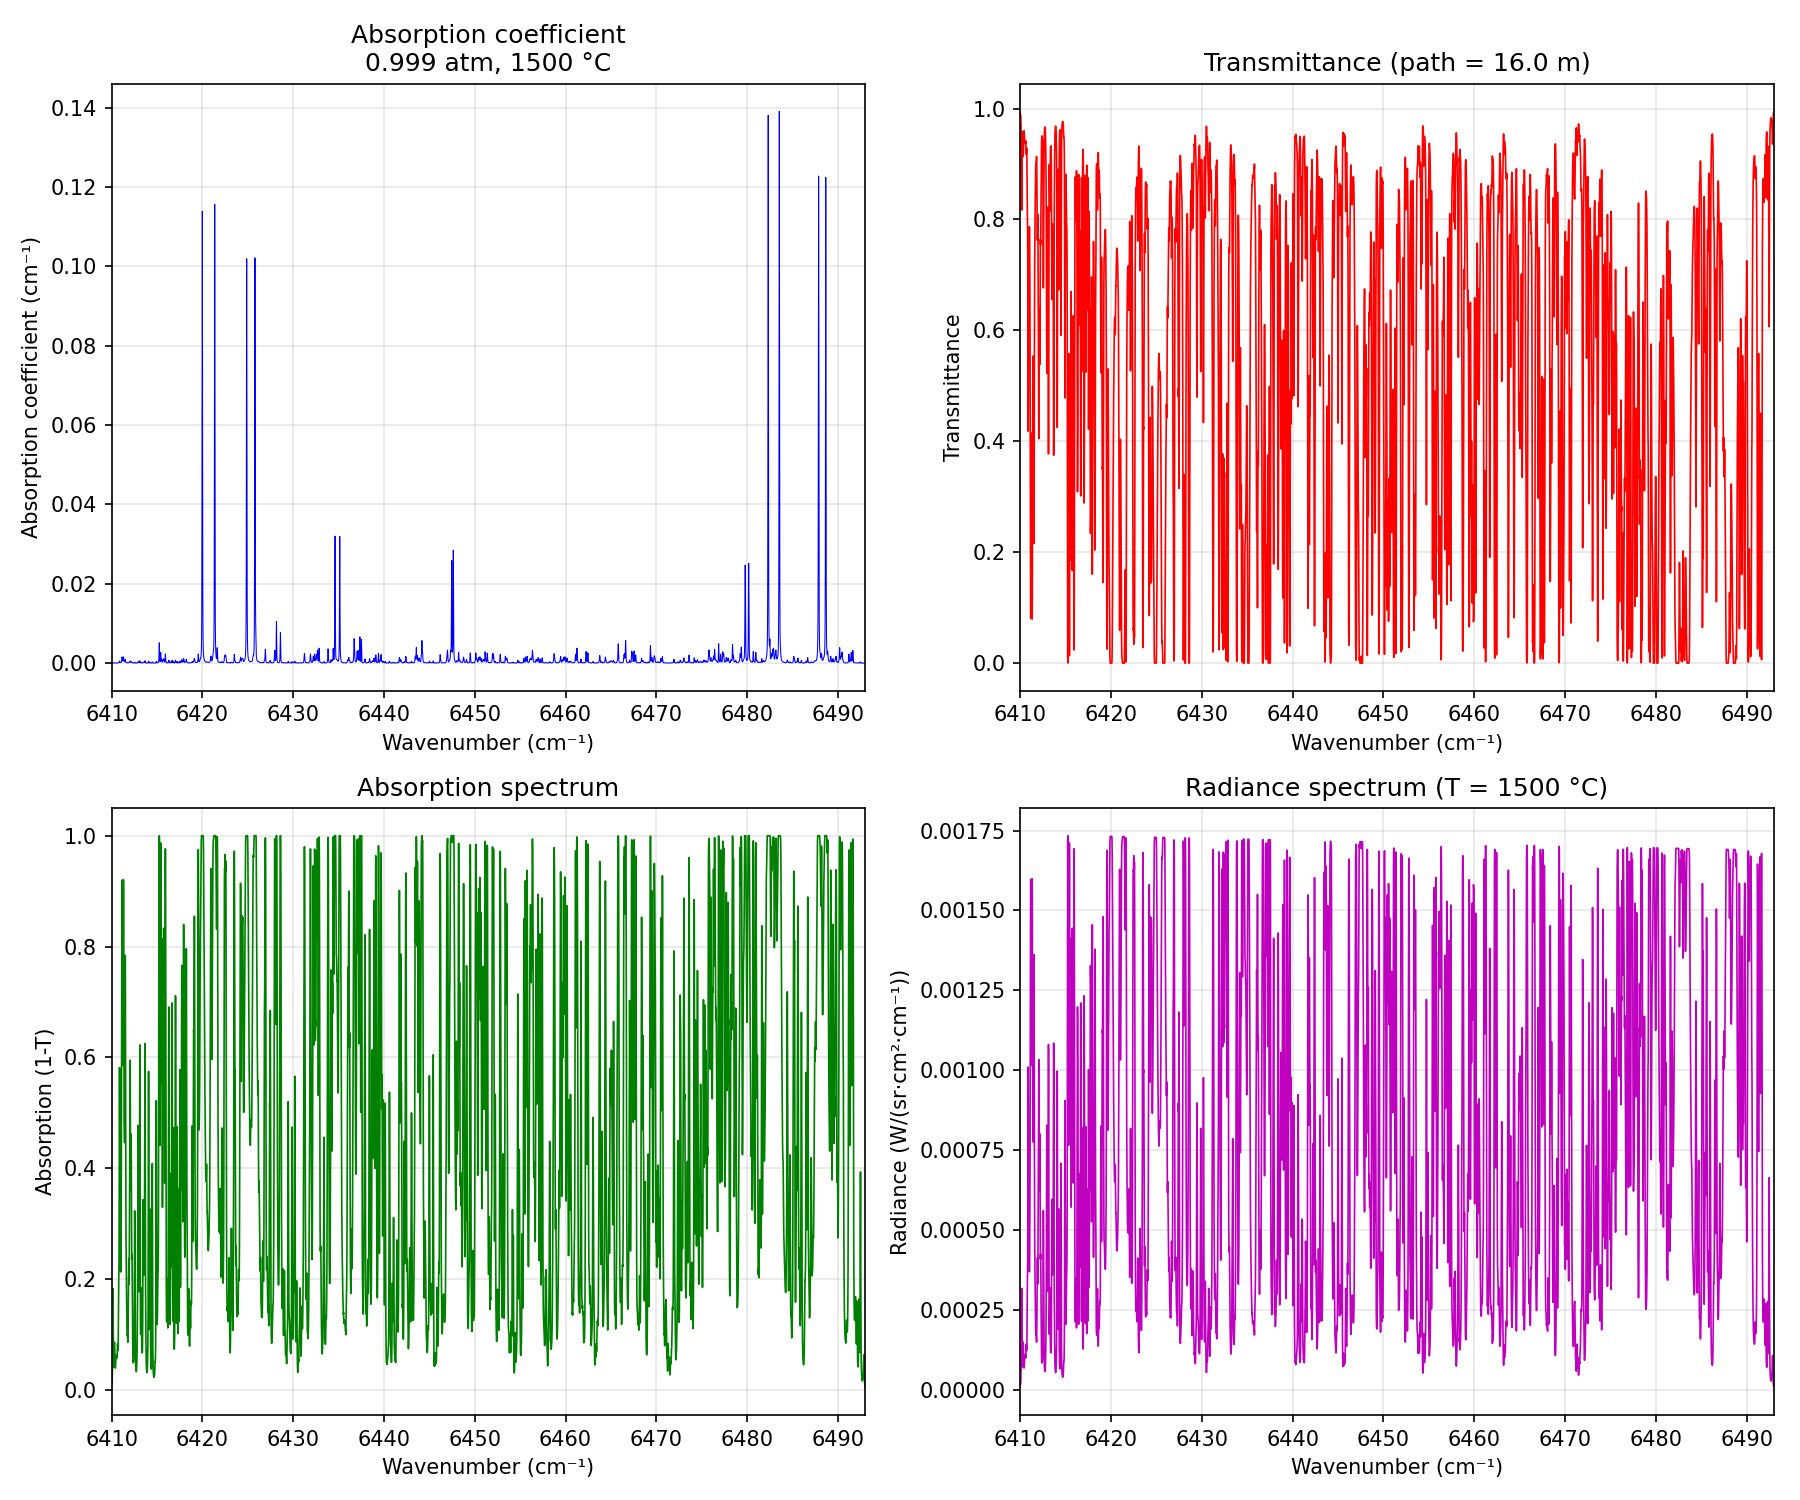
\includegraphics[width=0.72\textwidth]{figures/spectra_full.png}
  \caption{1.5\,$\mu$m 波段四合一光谱仿真图}
  \label{fig:spectra}
\end{figure}

\textbf{关键技术决策已定：}扫描频率统一 100\,kHz；APD 偏置修正为 25--175\,V；TIA 升级路线选定 OPA855（GBW 8\,GHz）；环形器暂缓、以裸光纤端面反射替代先行打通链路；锅炉工况仿真基准（1773\,K/0.999\,atm/16\,m）。

\textbf{应用侧基础（对应研究内容四、五）：}343 线锅炉适配与现场测量方案开展中（E 子课题），激光系统已进驻校外集装箱场地；711 线完成反应器总体设计定稿（内筒 $\phi$220$\times$15/外筒 $\phi$250$\times$5、允许工作压力 17.3\,MPa、散热与冷却水核算）、密封方案（法兰--定位环--紫铜垫圈）、蓝宝石棒状光学窗口设计、单相 30 套星形接法温控方案；三份专利交底书已定稿（超音速引射器煤粉进样/可更换中心管固定床/小型连续气化系统）。

\textbf{遇到的问题与解决思路：}首次 APD 调试因偏置电压操作不当疑似损坏器件——已转化为标准操作卡（黑胶带遮挡测暗电流$\rightarrow$逐步引入光信号）并撰写实践博客；集装箱场地上位机连接异常——取回已验证上位机替换排查（进行中）；课题组激光器运输损坏事件——本课题设备转运一律执行减振包装规定。

% ============================================================================
%  五、工作计划
% ============================================================================
\section{工作计划}

按三年制培养（2025.09--2028.06）编排：

\begin{table}[htbp]
  \centering
  \caption{论文工作计划（进度安排）}
  \begin{tabular}{p{1.0cm}p{2.9cm}p{5.2cm}p{4.2cm}}
    \toprule
    阶段 & 时间 & 研究内容 & 阶段成果 \\
    \midrule
    一 & 2025.09--2026.06 & 课程学习与文献调研；器件选型采购；光谱仿真；光源链路搭建与出光验证（已基本完成） & 选线仿真数据库；系统核心器件齐备 \\
    二 & 2026.07--2026.12 & 接收链路升级（OPA855）与回波信号采集；单端光路方案定型；crossflow 平台双模式验证；开题报告（2026.10） & 系统样机；实验室验证数据；开题通过 \\
    三 & 2027.01--2027.06 & 锅炉集装箱场地与电站现场测量；小论文一（光源链路+实验室验证）撰写投稿 & 现场实测数据；小论文投稿 \\
    四 & 2027.07--2027.12 & 711 高压反应器窗口耦合与高压气氛实验；中期考核；专利提交；小论文二（现场/高压应用） & 中期报告；专利受理；第二篇小论文 \\
    五 & 2028.01--2028.03 & 学位论文撰写与修改 & 学位论文初稿 \\
    六 & 2028.04--2028.06 & 论文送审、修改、答辩 & 学位论文定稿；通过答辩 \\
    \bottomrule
  \end{tabular}
\end{table}

\textbf{预期成果：}
\begin{enumerate}
  \item 系统成果：1.5\,$\mu$m 单端 TDLAS 测温系统样机一套（100\,kHz 扫描、亚毫秒温度反演、单侧安装）；
  \item 学术论文：硕士学位论文 1 篇；期刊小论文 2--3 篇（小论文一"光源链路开发与实验室验证"目标 Applied Optics / Measurement Science and Technology / Optics Express，构想稿已成文；应用篇视现场与高压实验进展）；
  \item 知识产权：发明专利 1--3 项（711 三份交底书已定稿，出图后即报）；
  \item 数据资产：1.5\,$\mu$m 波段 H$_2$O 高温（含高压展宽）吸收线选择与反演数据库一套。
\end{enumerate}

% ============================================================================
%  参考文献
% ============================================================================
\section{主要参考文献}

\begin{thebibliography}{18}
\small
\bibitem{goldenstein2017} Goldenstein C S, Spearrin R M, Jeffries J B, et al. Infrared laser-absorption spectroscopy for in-situ combustion diagnostics: status and outlook[J]. Measurement Science and Technology, 2017, 28(5): 052001.
\bibitem{melin2017} Melin S T, Wang Z, Neal N J, et al. Single-ended retroreflection sensors for absorption spectroscopy in high-temperature environments[J]. Applied Physics B, 2017, 123(4): 119.
\bibitem{zhou2018} Zhou Y, Mathews G F, Goldenstein C S. Compact, fiber-coupled, single-ended laser-absorption-spectroscopy sensors for high-temperature environments[J]. Applied Optics, 2018, 57(25): 7117-7126.
\bibitem{peng2016} Peng W Y, et al. Single-ended mid-infrared laser-absorption sensor for simultaneous in situ measurements of H$_2$O, CO$_2$, CO, and temperature in combustion flows[J]. Applied Optics, 2016, 55(33): 9347.
\bibitem{peng2019a} Peng W Y, et al. Single-ended sensor for thermometry and speciation in shock tubes using native surfaces[J]. IEEE Sensors Journal, 2019, 19(13): 4954-4961.
\bibitem{peng2019b} Peng W Y, et al. Single-ended mid-infrared laser-absorption sensor for time-resolved measurements of water concentration and temperature within the annulus of a rotating detonation engine[J]. Proceedings of the Combustion Institute, 2019, 37(2): 1435-1443.
\bibitem{hansemann2024} Hansemann C, et al. Towards a spatially resolved, single-ended TDLAS system for characterizing the distribution of gaseous species[J]. Scientific Reports, 2024, 14(1): 11708.
\bibitem{luo2024} Luo L, Li T, Zhao R, et al. Measurements of temperature downstream of the stratified swirl burner by a single-ended TDLAS sensor[C]. Optica Sensing Congress, 2024: LM1E.2.
\bibitem{chao2013} Chao X, Jeffries J B, Hanson R K. Real-time, in situ, continuous monitoring of CO in a pulverized-coal-fired power plant with a 2.3\,$\mu$m laser absorption sensor[J]. Applied Physics B, 2013, 110(3): 359-365.
\bibitem{li2020} Li J, et al. In situ, portable and robust laser sensor for simultaneous measurement of ammonia, water vapor and temperature in denitrification processes of coal fired power plants[J]. Sensors and Actuators B: Chemical, 2020, 305: 127533.
\bibitem{zhou2005} Zhou H C, et al. Experimental investigations on visualization of three-dimensional temperature distributions in a large-scale pulverized-coal-fired boiler furnace[J]. Proceedings of the Combustion Institute, 2005, 30(1): 1699-1706.
\bibitem{wang2020} Wang Z, Zhou W, Yan J, et al. Application of 2D temperature measurement to a coal-fired furnace using CT-TDLAS[J]. Measurement Science and Technology, 2020, 31(3): 035203.
\bibitem{li2024} Li K, et al. Simultaneous determination of 2-D distributions of temperature and absorption coefficient in large-scale pulverized-coal-fired boilers by flame images processing[J]. Proceedings of the Combustion Institute, 2024, 40(1): 105421.
\bibitem{ouyang1998} Ouyang S, Yeasmin H, Mathews J. A pressurized drop-tube furnace for coal reactivity studies[J]. Review of Scientific Instruments, 1998, 69(8): 3036-3041.
\bibitem{sun2013} Sun K, Chao X, Sur R, et al. TDL absorption sensors for gas temperature and concentrations in a high-pressure entrained-flow coal gasifier[J]. Measurement Science and Technology, 2013, 24(12): 125203.
\bibitem{sun2014} Sun K, Sur R, Jeffries J B, et al. Application of wavelength-scanned wavelength-modulation spectroscopy H$_2$O absorption measurements in an engineering-scale high-pressure coal gasifier[J]. Applied Physics B, 2014, 117(1): 411-421.
\bibitem{xie2017} 谢和平, 高峰, 鞠杨, 等. 深地煤炭资源流态化开采理论与技术构想[J]. 煤炭学报, 2017, 42(3): 547-562.
\bibitem{xie2018} 谢和平, 鞠杨, 高峰, 等. 煤炭深部原位流态化开采的理论与技术体系[J]. 煤炭学报, 2018, 43(5): 1210-1219.
\end{thebibliography}

\clearpage

% ============================================================================
%  评分表（模板自带，留空待签）
% ============================================================================
\thispagestyle{empty}
\begin{center}
  {\heiti\large 山东科技大学硕士研究生学位论文开题报告评分表}
\end{center}

\renewcommand{\arraystretch}{1.5}
\begin{longtable}{|p{3.0cm}|p{1.6cm}|p{8.4cm}|p{1.8cm}|}
  \hline
  \heiti 评审项目 & \heiti 分值 & \heiti 评分标准 & \heiti 得分（百分制） \\
  \hline
  \multirow{3}{*}{一、选题依据} & \multirow{3}{*}{30 分} & 21--30 分：选题有较强的理论意义、实用价值，深刻的学术研究内涵。 & \\
  \cline{3-4}
  & & 11--20 分：选题有一定的理论意义、实用价值，有一定的学术研究内涵。 & \\
  \cline{3-4}
  & & 0--10 分：选题缺乏理论意义和实用价值。 & \\
  \hline
  \multirow{3}{*}{二、理论基础和专门知识} & \multirow{3}{*}{20 分} & 15--20 分：较好地掌握坚实宽广的理论基础和系统专业知识。 & \\
  \cline{3-4}
  & & 6--15 分：基本掌握坚实宽广的理论基础和系统专业知识。 & \\
  \cline{3-4}
  & & 5 分以下：未能掌握坚实宽广的理论基础和系统知识。 & \\
  \hline
  \multirow{3}{*}{三、选题难度及先进性} & \multirow{3}{*}{30 分} & 21--30 分：研究课题属本学科发展方向并居前沿位置，具有自己独特的思考，研究课题具有较强的先进性。 & \\
  \cline{3-4}
  & & 11--20 分：研究课题属本学科的发展方向，并具有先进性。 & \\
  \cline{3-4}
  & & 0--10 分：研究课题与本学科的发展方向先进性不明显，难度欠佳。 & \\
  \hline
  \multirow{3}{*}{四、文字表达} & \multirow{3}{*}{10 分} & 8--10 分：条理清晰，分析严谨，文笔流畅。 & \\
  \cline{3-4}
  & & 4--7 分：条理较好，层次分明，文笔较流畅。 & \\
  \cline{3-4}
  & & 3 分以下：写作能力较差。 & \\
  \hline
  \multirow{3}{*}{五、口头报告} & \multirow{3}{*}{10 分} & 8--10 分：论文严密、逻辑性强、表达清楚。 & \\
  \cline{3-4}
  & & 3--7 分：基本概念清晰、层次分明、表达较清楚。 & \\
  \cline{3-4}
  & & 3 分以下：表达较差。 & \\
  \hline
  \multicolumn{2}{|l|}{\heiti 总分} & & \\
  \hline
  \multicolumn{4}{|l|}{开题评审小组组成：} \\
  \multicolumn{4}{|l|}{\hspace{1em}组成 \hfill 姓名 \hfill 职称 \hfill 单位 \hfill 签字 \hfill} \\
  \multicolumn{4}{|l|}{\hspace{1em}导师 \hfill \hfill \hfill \hfill} \\
  \multicolumn{4}{|l|}{\hspace{1em}组长 \hfill \hfill \hfill \hfill} \\
  \multicolumn{4}{|l|}{\hspace{1em}成员 \hfill \hfill \hfill \hfill} \\
  \multicolumn{4}{|l|}{\hspace{1em}\hspace{6.5cm}年 \ \ 月 \ \ 日} \\
  \hline
\end{longtable}

\clearpage
\thispagestyle{empty}
\vspace*{0.5cm}
\begin{center}
  {\heiti\large 评审意见}
\end{center}

\renewcommand{\arraystretch}{1.6}
\begin{longtable}{|p{12.8cm}|}
  \hline
  \heiti 导师对本课题的评价 \\[3.5cm]
  \hline
  \hspace{6.2cm}导师签名 \ \ \ \ \ \ 年 \ \ 月 \ \ 日 \\
  \hline
  \heiti 评审小组的审查结论 \\[3.5cm]
  \hline
  \hspace{1.0cm}组长 \hfill \hspace{3.4cm}  \\
  \hspace{1.0cm}组员 \hfill \hspace{3.4cm}  \\
  \hspace{6.2cm}年 \ \ 月 \ \ 日 \\
  \hline
  \heiti 学科专业分委员会意见 \\[3.5cm]
  \hline
  \hspace{6.2cm}负责人签名 \ \ \ \ \ \ 年 \ \ 月 \ \ 日 \\
  \hline
\end{longtable}

\end{document}
